\documentclass[12pt]{article}
\usepackage{amsmath}
\usepackage{amssymb}
\usepackage[letterpaper,top=1.5in,bottom=1.25in,left=0.75in,right=0.75in,centering]{geometry}
\usepackage{fancyhdr}
\usepackage{enumerate}
\usepackage{lastpage}
\usepackage{multicol}
\usepackage{graphicx}
\usepackage{vwcol}
\reversemarginpar

\pagestyle{fancy}
\cfoot{Page \thepage \ of \pageref{LastPage}}\rfoot{}
\chead{MATH 1560}\lhead{Test \#1 Solutions}\rhead{September 19th, 2017}

\newcommand{\points}[1]{\marginpar{\hspace{24pt}[#1]}}
\newcommand{\skipline}{\vspace{12pt}}
%\renewcommand{\headrulewidth}{0in}
\headheight 30pt

\newcommand{\di}{\displaystyle}
\newcommand{\abs}[1]{\lvert #1\rvert}
\newcommand{\R}{\mathbb{R}}
\newcommand{\C}{\mathbb{C}}
\renewcommand{\P}{\mathcal{P}}
\DeclareMathOperator{\nul}{null}
\DeclareMathOperator{\range}{range}
\DeclareMathOperator{\spn}{span}
\newcommand{\len}[1]{\lVert #1\rVert}
\newcommand{\Q}{\mathbb{Q}}
\newcommand{\N}{\mathbb{N}}
\renewcommand{\L}{\mathcal{L}}
\newcommand{\dotp}{\boldsymbol{\cdot}}
\newenvironment{amatrix}[1]{%
  \left[\begin{array}{@{}*{#1}{c}|c@{}}
}{%
  \end{array}\right]
}
\newcommand{\bam}{\begin{amatrix}}
\newcommand{\eam}{\end{amatrix}}
\newcommand{\bbm}{\begin{bmatrix}}
\newcommand{\ebm}{\end{bmatrix}}

\begin{document}


 \begin{enumerate}
 \item  Evaluate the following limits:
\begin{enumerate}
 \item \begin{align*}
 \lim_{x\to 3} \frac{x^2-6x+9}{x^2-5x+6} & = \lim_{x\to 3}\frac{(x-3)(x-3)}{(x-2)(x-3)}\\
 & = \lim_{x\to 3}\frac{x-3}{x-2} = \frac{3-3}{3-2}=0.
\end{align*}  

 \item \begin{align*}
 \lim_{x\to 0}\frac{\tan(7x)}{x}& = \lim_{x\to 0}\frac{\sin(7x)}{x\cos(7x)}\\
 & = \lim_{x\to 0}\frac{\sin(7x)}{7x}\cdot\frac{7}{\cos(7x)}\\
 & = \lim_{x\to 0}\frac{\sin(7x)}{7x}\cdot \lim_{x\to 0}\frac{7}{\cos(7x)}\\
 & = (1)\frac{7}{1} = 7.
 \end{align*} 

 \item \begin{align*}
 \lim_{x\to 1}\frac{\sqrt{x}-1}{x^2-1} & = \lim_{x\to 1}\frac{\sqrt{x}-1}{(x-1)(x+1)}\cdot\frac{\sqrt{x}+1}{\sqrt{x}+1}\\
 & = \lim_{x\to 1}\frac{x-1}{(x-1)(x+1)(\sqrt{x}+1)}\\
 & = \lim_{x\to 1}\frac{1}{(x+1)(\sqrt{x}+1)}\\
 & = \frac{1}{(1+1)(1+1)} = \frac{1}{4}.
 \end{align*}
Alternative solution: factor the $x-1$ in the denominator as $(x-1)=(\sqrt{x}-1)(\sqrt{x}+1)$.
\begin{align*}
\lim_{x\to 1}\frac{\sqrt{x}-1}{x^2-1}& = \lim_{x\to 1}\frac{\sqrt{x}-1}{(\sqrt{x}-1)(\sqrt{x}+1)(x+1)}\\
& = \lim_{x\to 0}\frac{1}{(\sqrt{x+1})(x+1)} = \frac{1}{4}.
\end{align*}
\end{enumerate}
\newpage

\item The graph of a function $f$ is given below: 

\begin{center}
 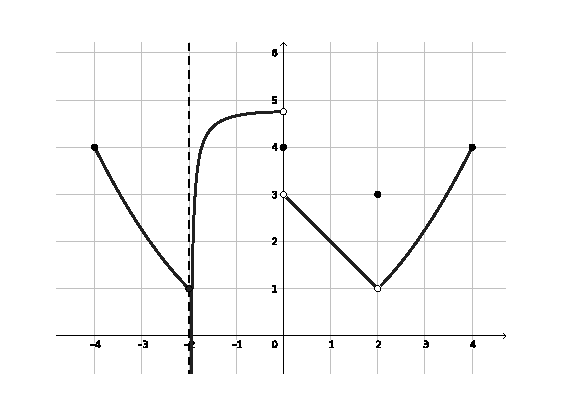
\includegraphics[width=4.5in]{FE-3}
\end{center}


Determine the following values (write DNE if something does not exist):
\begin{multicols}{2}
\begin{enumerate}
 \item The domain of $f$: \underline{\hspace{1cm}$[-4,4]$\hspace{1cm}}
 
 \bigskip
 
 
 \bigskip
 
 \item $\di\lim_{x \to -2^-}f(x)$: \underline{\hspace{1cm}$1$\hspace{1cm}}
 
 \bigskip

 \bigskip
 
 \item $\di \lim_{x\to -2^+}f(x)$: \underline{\hspace{1cm}$-\infty$\hspace{1cm}}  
 
 \bigskip
 
 \bigskip
 
 \item $\di \lim_{x\to -2}f(x)$: \underline{Does not exist}
 
 \bigskip
 
 \bigskip
 
 \item $f(-2)$: \underline{\hspace{1cm}$1$\hspace{1cm}}

\columnbreak


 \item $\di \lim_{x \to 2^-}f(x)$: \underline{\hspace{1cm}$1$\hspace{1cm}}
 
 \bigskip
 
 \bigskip
 
 \item $\di \lim_{x\to 2^+}f(x)$: \underline{\hspace{1cm}$1$\hspace{1cm}} 

\bigskip

\bigskip

 \item $\di \lim_{x\to 2}f(x)$: \underline{\hspace{1cm}$1$\hspace{1cm}}
 
 \bigskip
 
 \bigskip
 
\item $f(2)$: \underline{\hspace{1cm}$3$\hspace{1cm}}
\end{enumerate}
\end{multicols}
\end{enumerate}
\end{document}